\section{Explainability}
\textbf{Interpretability} (or \textbf{explainability}) refers to how well a human can understand the reasons behind a model's prediction. A highly interpretable model makes it easier to identify not only how decisions are made, but also potential biases in the model or the data.

A \textbf{black box} model has internal workings that are unknown or too complex to interpret, such as deep neural networks, SVMs, and ensemble methods. In contrast, models like decision trees, linear and logistic regression are interpretable by design.

\vspace{0.3cm}
\noindent
\textbf{Interpretability methods can be classified as:}
\begin{itemize}
    \item \textbf{Intrinsic/Post-hoc:}  
    Intrinsically interpretable models (e.g., decision trees) are simple by design. Post-hoc methods explain any model after training, regardless of its complexity.
    \item \textbf{Model-specific/Model-agnostic:}  
    Model-specific techniques work only for particular models (e.g., regression coefficients), while model-agnostic ones (e.g., SHAP, LIME) can be applied to any model but may not capture true causal reasoning.
    \item \textbf{Global/Local:}  
    Global methods explain overall model behavior, while local ones focus on individual predictions.
\end{itemize}

Intrinsic methods are always global and model-specific. Post-hoc methods can be any combination.

\begin{table}[H]
    \centering
    \begin{tabular}{|c|c|}
    \hline
        \textbf{Data type} & \textbf{Techniques} \\
        \hline
        \textbf{Tabular Data} & Feature importance, decision trees \\
        \hline
        \textbf{Image Data} & Saliency maps, segmentation maps \\
        \hline
        \textbf{Text Data} & Sentence highlighting, attention mechanisms \\
        \hline
    \end{tabular}
\end{table}

For all data types, techniques like \textit{prototypes} and \textit{counter-examples} can be used.

\begin{itemize}
    \item \textit{Saliency Maps:} pixel brightness indicates importance. These can be computed per-pixel or per-segment (superpixels).

    \item \textit{Sentence Highlighting:} Words in a sentence are assigned scores showing their impact on the model's prediction, helping understand which parts of the text were influential.
\end{itemize}

\begin{figure}[H]
    \centering
    \begin{minipage}{0.45\textwidth}
        \centering
        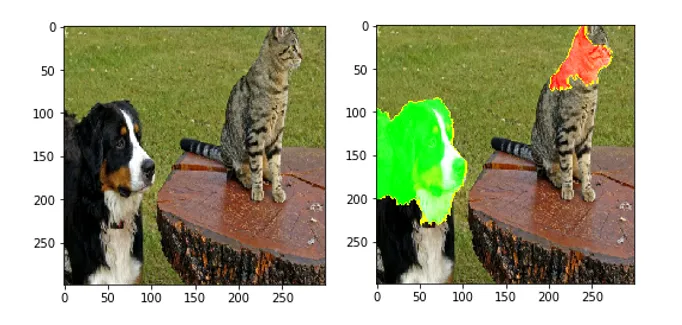
\includegraphics[width=\textwidth]{img/saliency_map_dog_cat.png}
        \caption{Saliency map: green areas support the \textit{dog} class; red areas oppose it.}
    \end{minipage} \hfill
    \begin{minipage}{0.45\textwidth}
        \centering
        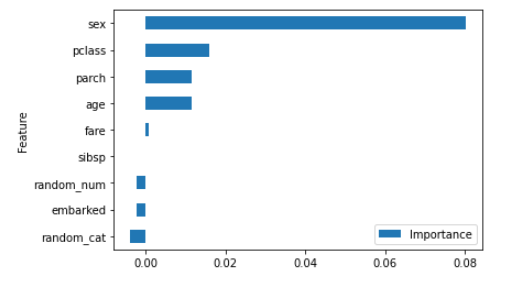
\includegraphics[width=\textwidth]{img/feature_importance.png}
        \caption{Feature importance plot: positive means positive impact on prediction.}
    \end{minipage}
\end{figure}

\subsection{TREPAN}
TREPAN is a global explainer designed to extract symbolic representations from trained neural networks, although it can be applied to any black box model. It works by querying the neural network and building a decision tree that approximates the network's behavior using \textbf{$m$-of-$n$ rules}. These rules are Boolean expressions, where an integer threshold $m$ and a set of $n$ Boolean conditions define the rule. The rule is satisfied if at least $m$ of the $n$ conditions are true.

One limitation of traditional decision trees is that at lower depths, splits are less meaningful because they rest on a small number of training instances. TREPAN addresses this by selecting as many instances as needed to build a split-condition rule. Instead of predicting the original label directly, it learns to predict the label returned by the black box model.

When selecting a split at a given node, the oracle receives the list of all previously selected splits along the path from the root to that node. This context restricts the feature values considered when constructing the rule, so the splits stay relevant to the decisions made earlier in the tree. As a result, TREPAN builds more accurate and interpretable trees that better approximate complex black box models like neural networks.
\subsection{Local Interpretable Model-Agnostic Explanations (LIME)}
\textbf{LIME} (Local Interpretable Model-agnostic Explanations) is a local explainer that uses surrogate models, typically a logistic regressor with LASSO or Ridge regularization, to approximate the predictions of a black-box model. While the global decision boundary of a model may be complex, LIME focuses on the neighborhood of a single instance, where the model's behavior is simpler and more interpretable. This is achieved by auditing the black-box model around the given instance and learning a local decision.

LIME works by perturbing the data instance, generating a new dataset composed of perturbed instances and their corresponding predictions by the black-box model. An interpretable surrogate model (such as local linear regression) is then trained on this new dataset, with the data points weighted by their proximity to the instance of interest. This surrogate should approximate the original model well near that instance, though not globally. This local accuracy is called \textbf{local fidelity}.

For tabular data, instances are perturbed by changing the values of the features, sampling from a normal distribution with mean and standard deviation taken from the feature itself. Each feature is assigned an importance score, describing how much each feature contributes (positively or negatively) to the prediction.

For image or text data, LIME uses a different approach. For images, it transforms the image into interpretable superpixel vectors, which represent the presence or absence of certain pixels. A synthetic neighborhood is created by randomly perturbing these superpixels and labeling them with the black-box predictions. A linear regression model is then trained on this synthetic data, and the surrogate assigns weights to each superpixel based on its proximity to the instance being explained. This method works better than perturbing single pixels, as changes to individual pixels may not significantly alter the prediction.

\subsection{LORE}
\textbf{LORE} (LOcal Rule-based Explainer) extends LIME by using a decision tree as the surrogate model. It generates synthetic instances through a genetic procedure that considers both instances sharing the label of the target and instances with a different one. Each local explanation is a pair: a logic rule describing the decision-tree path that explains the classification, and a set of \textbf{counterfactual rules}, listing the conditions to change for a different prediction. LORE applies to text and image data using the same representations as LIME.

\subsection{SHAP}
\textbf{Shapley values} come from coalitional game theory and fairly distribute a prediction across the features. They explain the gap between a specific prediction and the average prediction by measuring each feature's marginal contribution across all possible coalitions. Enumerating every coalition is expensive, so in practice we compute the contributions over a sampled subset of coalitions.

\textbf{SHAP} (SHapley Additive exPlanations) is a model-agnostic method based on Shapley values, explaining a given instance's prediction by calculating each feature's contribution. In SHAP, the explanation is represented as a linear model:
\begin{equation*}
    g(z') = \phi_0 + \sum_{i=1}^M \phi_i z_i'
\end{equation*}
where $g$ is the explanation model, $z'$ is the coalition vector, $M$ is the number of simplified input features, and $\phi_i$ is the Shapley value for feature $i$. This assigns an importance value to each feature based on its contribution to the prediction.

\subsection{Integrated Gradients}
\textbf{Integrated Gradients} accumulates the gradients along the path from a baseline (e.g., a black image for images, or a zero embedding vector for text) to the input instance. The integrated gradient of each input is the cumulative sum of these gradients, and the result can be visualized (e.g., as saliency maps for images).

\subsection{Instance-Based Explanations}
Instance-based explanation methods generate or select instances to explain black box model behavior, typically focusing on local explanations. These methods are useful when the input is human-readable, such as tabular data, images, or short text. Instance-based methods can be divided into two main groups:

\begin{itemize}
    \item \textbf{Prototypes}: representative instances of the same class as the instance being explained, including \textbf{criticisms} (poorly represented instances) and \textbf{influential instances} (instances that significantly influenced the model's prediction).
    
    \item \textbf{Counterfactuals}: representative instances from a different class, showing the smallest change needed to alter the prediction to a different class (e.g., the opposite class in a binary task).
\end{itemize}

Many methods generate counterfactuals, and they fall into two families: optimization-based and heuristic-based approaches.

\paragraph{Optimization-based Methods}

A simple approach is trial-and-error, randomly altering feature values until the desired outcome is achieved. A more refined method uses a loss function to find the optimal counterfactual:

\[
L(x, x', y', \lambda) = \lambda \cdot (\hat{f}(x') - y')^2 + d(x, x')
\]

Here, the first term represents the squared difference between the counterfactual's prediction and the desired outcome, while the second term is the distance between the original instance \( x \) and the counterfactual \( x' \), typically measured using Manhattan distance. \( \lambda \) is a regularization term that balances these two components.

The steps to generate a counterfactual are as follows:
\begin{enumerate}
    \item Choose the instance \( x \), desired outcome \( y' \), tolerance \( \epsilon \), and regularization term \( \lambda \).
    \item Sample a random instance as the initial counterfactual.
    \item Optimize the loss function, adjusting the counterfactual iteratively until the prediction meets the desired outcome within the tolerance.
\end{enumerate}

Alternatively, a tolerance \( \epsilon \) can be used instead of a fixed \( \lambda \):

\[
|\hat{f}(x') - y'| \leq \epsilon
\]

\paragraph{DICE (Diverse Counterfactual Explanations)}

The \textbf{DICE} method addresses diversity and similarity by solving an optimization problem with penalization terms. It generates \( k \) counterfactuals that are both plausible and diverse:

\[
C(x) = \arg \min_{c_1, \dots, c_k}\, \left( \frac{1}{k}\sum_{i=1}^k L(f(c_i), y') + \frac{\lambda_1}{k}\sum_{i=1}^k d(c_i, x) - \lambda_2 \cdot \textit{dpp-diversity}(c_1, \dots, c_k) \right)
\]

Here, \textit{dpp-diversity} measures the diversity among the counterfactuals.

\paragraph{Heuristic-based Methods}

Heuristic strategies are faster but may not find the optimal solution. They iteratively update the counterfactual based on local improvements. Common methods include:

\begin{itemize}
    \item \textbf{SEDC} (Search for Explanations for Document Classification): a brute-force approach that removes one word at a time and observes the output, then progresses to combinations of two or more words.
    \item \textbf{GSG} (Growing Spheres Generation): a generative approach that creates synthetic instances around the original instance \( x \) in spherical layers, seeking a counterfactual within these regions. It may, however, generate unnecessary instances and might not find the optimal solution.
    \item \textbf{Instance-based Approaches}: These methods search for counterfactuals within a reference population. Examples include:
    \begin{itemize}
        \item \textbf{NNCE} (Nearest-Neighbor Counterfactual Explainer): Selects counterfactuals based on similarity to \( x \) and a different class label, using a nearest-neighbor search.
        \item \textbf{CBCE} (Case-Based Counterfactual Explainer): A refinement of NNCE, it defines an \textbf{explanation case} (\( xc \)) as a pair of similar instances with different labels, aiding in efficient counterfactual generation.
    \end{itemize}
\end{itemize}
